\documentclass[aspectratio=169]{beamer}
\usepackage{color,amsmath}
\usepackage{subfigure}
\usepackage{booktabs}
\usepackage{framed}
\usepackage{comment}

\usepackage{hyperref}
\hypersetup{
    colorlinks=true,
    linkcolor=blue,
    filecolor=magenta,      
    urlcolor=cyan,
}

%%%%%%%%%%%%%%%%%%%%%%%%%%
\title[]{\textcolor{gray}{[What, why, and which experiments?]}, \newline [Moving beyond simple experiments], \textcolor{gray}{[Making it happen], \newline [Zero variable cost data and MusicLab], [3 Rs]}}
\author[]{Matthew J. Salganik\\Department of Sociology\\Princeton University}
\date[]{
\begin{flushright}

\includegraphics[width=0.1\textwidth]{figures/cc-by.png}
\end{flushright}
}
\begin{document}
%%%%%%%%%%%%%%%%%%%%%%%%%%
\frame{\titlepage}
%%%%%%%%%%%%%%%%%%%%%%%%%%
\begin{frame}

\begin{columns}
\begin{column}{.40\textwidth}
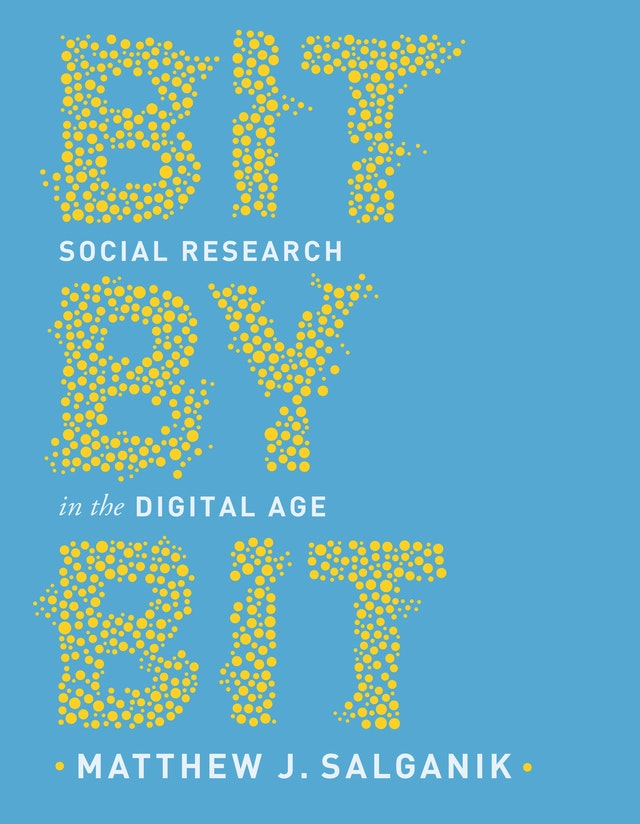
\includegraphics[width=\textwidth]{figures/salganik_bit_2018_cover}
\end{column}%

\hfill%

\begin{column}{.60\textwidth}
1) Introduction \\
2) Observing behavior \\
3) Asking questions \\
\textcolor{blue}{4) Running experiments} \\
5) Mass collaboration \\
6) Ethics \\
7) The future \\
\end{column}%
\end{columns}

\end{frame}
%%%%%%%%%%%%%%%%%%%%%%
\begin{frame}

\Large{
\begin{center}
Optimization experiments vs  Understanding experiments
\end{center}
}

\end{frame}
%%%%%%%%%%%%%%%%%%%%%%%
\begin{frame}

\Large{
\begin{center}
Optimization experiments + Understanding experiments
\end{center}
}

\end{frame}
%%%%%%%%%%%%%%%%%%%%%%%
\begin{frame}

\begin{figure}
  \centering
  \includegraphics[width = 0.9\textwidth]{figures/schultz_constructive_2007_title}
\end{figure}

\vfill
\tiny{\url{http://dx.doi.org/10.1111/j.1467-9280.2007.01917.x}}

\end{frame}
%%%%%%%%%%%%%%%%%%%%%%%
\begin{frame}

\begin{figure}
  \centering
  \includegraphics[width = \textwidth]{figures/energy_peers_no_emoticon}
\end{figure}

\vfill
\tiny{Figures from Allcott (2011)}

\end{frame}
%%%%%%%%%%%%%%%%%%%%%%%%
\begin{frame}

\begin{figure}
  \centering
  \only<1>{\includegraphics[width = 0.5\textwidth]{figures/schultz_constructive_2007_1panel}}
  \only<2>{\includegraphics[width = 0.8\textwidth]{figures/schultz_constructive_2007_2panel}}
\end{figure}

\end{frame}
%%%%%%%%%%%%%%%%%%%%%%%%
\begin{frame}

\begin{figure}
  \centering
  \only<1>{\includegraphics[width = \textwidth]{figures/allcott_social_2011_fig1}}
  \only<2>{\includegraphics[width = \textwidth]{figures/allcott_social_2011_fig1_arrow}}
\end{figure}

\vfill
\tiny{Figures from Allcott (2011)}

\end{frame}
%%%%%%%%%%%%%%%%%%%%%%%%
\begin{frame}

\begin{figure}
  \centering
  \includegraphics[width = \textwidth]{figures/schultz_constructive_2007_23panel}
\end{figure}

\end{frame}
%%%%%%%%%%%%%%%%%%%%%%%%
\begin{frame}

If you want to move beyond simple experiments:
\begin{itemize}
\item Validity
\item Heterogeneity of treatment effects
\item Mechanisms
\end{itemize}

\end{frame}
%%%%%%%%%%%%%%%%%%%%%%%%%%%
\begin{frame}

Validity \pause
\begin{itemize}
\item statistical conclusion validity
\item internal validity
\item construct validity
\item external validity
\end{itemize}

\end{frame}
%%%%%%%%%%%%%%%%%%%%%%%%%%%
\begin{frame}

Heterogeneous treatment effects \pause
\begin{itemize}
\item lots of people, lots of pre-treatment information: stop treating people like widgets
\pause
\item beware of fishing (preregistration, data splits)
\pause
\item Lots of new methods in this area
\end{itemize}

\end{frame}
%%%%%%%%%%%%%%%%%%%%%%%%%%%
\begin{frame}

Mechanisms \pause
\begin{itemize}
\item Eating citrus prevents scurvy \pause
\item The mechanism through which citrus prevents scurvy vitamin C
\end{itemize}

\begin{itemize}
\item Not as easy as scurry and limes, ``Enough already about black box experiments''  \textcolor{blue}{\href{http://dx.doi.org/10.1177/0002716209351526}{Green et al (2010)}}
\pause
\item Experiments specifically designed to test mechanisms: \textcolor{blue}{\href{http://dx.doi.org/10.1257/jep.25.3.17}{Ludwig et al (2011)}}, \textcolor{blue}{\href{http://dx.doi.org/10.1111/j.1467-985X.2012.01032.x}{Imai et al (2012)}}, \textcolor{blue}{\href{http://dx.doi.org/10.1016/j.jesp.2015.09.012}{Pirlott and MacKinnon (2016)}}
\end{itemize}

\end{frame}
%%%%%%%%%%%%%%%%%%%%%%%%%%%
\begin{frame}

\Large{
\begin{center}
Optimization experiments + Understanding experiments
\end{center}
}

\end{frame}
%%%%%%%%%%%%%%%%%%%%%%%
\frame{\titlepage}
%%%%%%%%%%%%%%%%%%%%%%%




\end{document}
